\section{Uvod}
U ovom radu je na DE1-SoC razvojnom sistemu implementiran jednostavan hardver u FPGA, portovan je Linuks operativni sistem i napisan je drajver za pristup registrima i prihvatanje prekida iz FPGA. 

\subsection{Sistemi na čipu sa FPGA}
Sa sve većim mogućnostima namenskih sistema došlo je do popularizacije sistema na čipovima (SoC - \textit{System on Chip}) koji integrišu mikroprocesore sa više jezgara, memorije na čipu, mnogobrojne periferije i transivere, kao i FPGA (\textit{Field Programmable Gate Array}).

Ova tehnologija daje dizajneru sistema veliku slobodu i mogućnosti, a zadršava se klasičan postupak projektovanja namenskih sistema. Uz to se ostvaruje veća integracija, manja potrošnja, manja površina štampane ploče (PCB - \textit{Printed Circuit Board}) i veći protok podataka između procesora i FPGA dela. 

Uobičajena primena ovih sistema je implementacija specifičnih akceleratora koji ubrzavaju izvršavanje algoritama i implementacija specifičnih programabilnih interfejsa ka spoljnom svetu. Sve zrelije tehnologije kao što su OpenCL, Vivado HLS, Matlab HDL Coder omogućavaju kompatibilnost dizajna softvera na visokom nivou i implementiranog hardvera na niskom nivou.

SoC FPGA sistemi najčešće sadrže ARM mikroprocesor. Aplikacije na mikroprocesoru bez operativnog sistema (\textit{baremetal application}) nude jednostavno pisanje koda i uštedu na resursima. Za kompleksnije aplikacije koriste se operativni sistemi (OS) i time se olakšava integrisanje mrežnih protokola, rad sa multimedijalnim sadržajima, kriptografskim bibliotekama kao i mnoge druge mogućnosti koje su dostupne kao \textit{open-source} softver. Kada je potrebno garantovati reakciju u određenom vremenu na neki spoljni događaj veliki operativni sistemi nisu dobro rešenje i koriste operativni sistemi u realnom vremenu (RTOS - \textit{Real time operating system}).

Hardver u FPGA se projektuje upotrebom nekog od dva popularna jezika za opis hardvera - Verilog i VHDL (\textit{Very High Speed Integrated Circuit Hardwer Description Language}). Pored toga neophodni su softverski alati za specifični uređaj, koje obezbeđuje sam proizvođač uređaja. Dodatno ovi alati olakšavaju dizajn upotrebom IP(\textit{Intelectual Property}) blokova, generisanjem raznih izlaznih fajlova koji opisuju projektovani hardver na standardni način i koriste se prilikom razvoja softvera.

\subsection{Opis DE1-SoC}

U ovom radu korišćen je DE1-SoC razvojni sistem koji se vrlo često upotrebljava u edukativne svrhe. Razvojni sistem je zasnovan na čipu iz familije Cyclone V kompanije Intel (ranije Altera).

U nastavku su navedene samo osobine razvojnog sistema koje se tiču ovog rada, a detaljniji opis se moze pronaći u dokumentu zvaničnoj dokumentaciji proizvođača []
dodati referencu: \verb+https://www.terasic.com.tw/cgi-bin/page/archive.pl?Language=English&CategoryNo=205&No=836&PartNo=4 +
DE1-SoC User Manual(rev.E Board)
Terasic
\begin{itemize}
\item Sistem na čipu Cyclone V \texttt{5CSEMA5F31}
\item Memorija 1GB (2x256Mx16) DDR3 SDRAM povezana na HPS
\item Slot za Micro SD karticu povezan na HPS
\item UART na USB (USB Mini-B konektor)
\item 5 debaunsiranih tastera (FPGA x4, HPS x1)
\item 11 LE dioda (FPGA x10, HPS x 1)
\item 12V DC napajanje
\end{itemize}

\subsection{Opis Altera Cyclone 5}
Altera Cyclone V je SoC FPGA koji se sastoji od dva dela(slika): procesorski deo (HPS -  \textit{Hard processor System}) i programabilni FGPA deo. HPS se sastoji od MPU (\textit{Microprocessor unit}) sa ARM Cortex-A9 MPCore sa dva jezgra i sledećih modula: kontroleri memorije, memorije, periferije, sistem interkonekcije, debug moduli, PLL moduli. FPGA deo se sastoji od sledećih delova: FPGA programabilna logika (\textit{look-up} tabele, RAM memorije, mnozači i rutiranje), kontrolni blok, PLL, kontroler memorije.

Svaki pin kućista je povezan na samo jedan od ova dva dela sistema, tako da HPS deo i FPGA deo ne mogu međusobno razmenjivati pinove.

\subsubsection{Konfigurisanje FPGA i pokretanje HPS}
Pri pokretanju HPS (boot) može da učita program iz FPGA dela, iz eksterne \textit{flash} memorije ili preko JTAG. FPGA ima mogućnost da se konfiguriše softverski iz HPS korišćenjem periferije FPGA Manager ili spoljnim programatorom. Kombinacije ovih mogucnosti daju nekoliko scenarija:
\begin{itemize}
\item nezavisno konfigurisanje FPGA i pokretanje HPS
\item konfigurisanje FPGA, zatim pokretanje HPS iz memorije koja se nalazi u FPGA
\item pokretanje HPS, zatim konfigurisanje FPGA iz HPS
\end{itemize}
DE1-SoC razvojni sistem dolazi sa integrisanim programatorom kojem se pristupa preko USB porta. Moguće je podesiti konfigurisanje FPGA spolja ili iz HPS upotrebom prekidača MSEL, dok se HPS uvek pokreće iz \textit{flash} memorije SD kartice.
(dodati tableu 3-2 iz de1soc user guide)

\subsubsection{HPS-FPGA interfejsi}
HPS-FPGA interfejsi su komunikacioni kanali između HPS i FPGA dela. U nastavku su nabrojani i opisani HPS-FPGA interfejsi:
\begin{itemize}
\item  FPGA-to-HPS bridge - magistrala visokih preformansi konfigurabilne sirine od 32,64 ili 128 bita. Na ovoj magistrali je FPGA master. Ovaj interfejs otkriva FPGA masterima ceo adresni prostor HPS dela.
\item HPS-to-FPGA bridge - magistrala visokih preformansi konfigurabilne sirine od 32,64 ili 128 bita. Na ovoj magistrali je HPS master a u FPGA se nalazi slave.
\item Lightweight HPS-to-FPGA - magistrala sirine 32 bita. HPS je master na ovoj magistrali. Ovaj interfejs manjeg protoka je namenjen za pristup statusnim i kontrolnim registrima periferijama implementiranim u FPGA delu.
\item FPGA manager - HPS periferja koja komunicira sa FPGA delom prilikom konfiguracije ili pokretanja (boot)
\item Prekidi - mogucnost povezivanja prekida iz FPGA na HPS kontroler prekida
\item HPS debug interfejs - omogućava da se debug mogućnosti prošire i na FPGA deo
\end{itemize}

Interfejsi koji su produžetak AXI magistrale na FPGA deo su FPGA-to-HPS bridge, HPS-to-FPGA bridge i Lightweight HPS-to-FPGA. Za povezivanje na ovu magistralu sa strane FPGA koristi se Avalon magistrala, stoga je neophodan AXI-Avalon bridge.

\subsubsection{Proces pokretanja HPS (boot)}
Pokretanje HPS je proces koji se obavlja u više koraka. Nakon izvršavanja svakog koraka se učitava i pokreće sledeći. Ovo je proces je sličan kod svih ARM procesora, a u nastavku je ukratko opisan za konkretnu platformu.

\begin{figure}[h!]
\centering
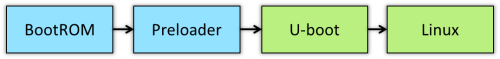
\includegraphics[scale=1.]{img/gsrd-boot.png}
\caption{Tok pokretana sistema}
\label{slika1:gsrd}
\end{figure}

Pri izlazu iz reset stanja procesor počinje izvrsavanje sa reset vektora iz memorije na čipu. Na adresi reset vektora je upisan Boot ROM progtam. Ovo je prvi korak u pokretanju HPS. \textit{Boot ROM} izvršava osnovna podešavanja procesora i dohvata \textit{preloader} iz NOR \textit{flash} memorije, NAND \textit{flash} memorije ili SD/MMC \textit{flash} memorije. Očitavaju se BSEL pinovi na osnovu kojih se određuje gde je smešten \textit{preloader}, zatim se inicijalizuje taj interfejs i učitava i pokreće \textit{preloader}. \textit{Boot ROM} softver proizvođača i ne može se menjati. 

\textit{Preloader} je prvi korak u pokretanju koji može da se konfiguriše. \textit{Preloader} obično izvršava inicijalizaciju SDRAM, dodatna podešavanja sitema, inicijalizaciju \textit{flash} kontrolera koji sadrži sledeći program (NAND, SD/MMC, QSPI) i zatim učitavanje programa u RAM memoriju i pokretanje.

Softver koji sledi nakon \textit{preloader}-a može biti \textit{baremetal} aplikacija ili \textit{bootloader}. \textit{Preloader} i svi prethodni programi se izvršavaju na prvom jezgru procesora dok je drugo u reset stanju. Naredni koraci mogu inicijalizovati drugo jezgro.

\textit{Bootloader} ima zadatak da podesi promenljive okruženja operativnog sistema, dohvati fajlove za pokretanje operativnog sistema (sa \textit{flash} memorije, putem \textit{Etherneta} preko TFTP protokola ili USB), konfigurise FPGA pruži konzolu za korisničke operacije. Neki od populatnih \textit{open-source} \textit{bootloader}-a su U-Boot i Barebox.

\subsection{Alati}
U nastavku će ukratko biti opisani korišćeni alati sa izdvojenim najvažnijim mogućnostima:
\begin{itemize}
\item Quartus Prime 18.0 - alat za razvoj hardvera na FPGA. Deo paketa je Platform Designer (ranije Qsys) koji u dizajn ukljucuje HPS, IP blokove i definiše povezanost ovih delova
\item \textit{Preloader Generator} (\texttt{bsp-editor} alat iz SoC EDS) - Generiše izvorni kod \textit{preloader}-a na osnovi izlaznih fajlova koji opisuju hardver
\item \textit{Device Tree Generator} (\texttt{sopc2dts} alat iz SoC EDS) - Generiše \textit{Device Tree} opis hardvera na osnovi izlaznih fajlova koji opisuju hardver
\item \textit{DE1-SoC Builder} - Generise prazan \textit{Quartus} projekat za DE1-SoC razvojni sistem
\item \textit{Linaro Toolchain} - koristi se za kompajliranje softvera
\end{itemize}

Na slici \ref{slika1:gsrd} je grafički prikazan tok projektovanja jednog SoCFPGA sistema.

\begin{figure}[h!]
\centering
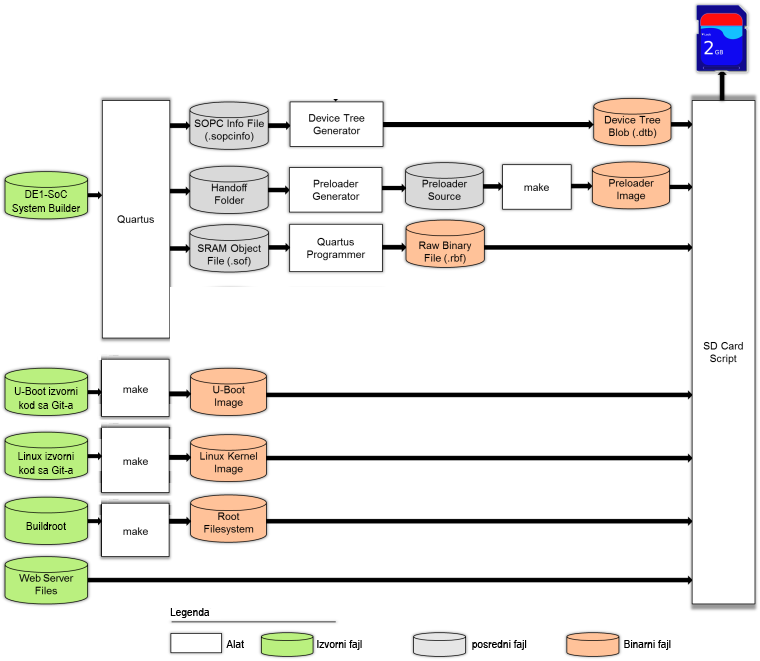
\includegraphics[scale=1.3]{img/gsrd-flow.png}
\caption{Tok projektovanja}
\label{slika1:gsrd}
\end{figure}

U nastavku su objašnjeni fajlovi koji se koriste pri projektovanju:
\begin{itemize}
\item \texttt{.qpf} - projektni fajl za Quartus. Ovaj fajl generiše DE1-SoC Builder
\item \texttt{.qsf} - skripta za podešavanje pinova. Ovaj fajl generiše DE1-SoC Builder
\item \texttt{.sdc} - skripta za podešavanje takta. Ovaj fajl generiše DE1-SoC Builder
\item \texttt{.v} - Verilog HDL izvorni kod
\item \texttt{.vhd} - VHDL izvorni kod
\item \texttt{.sof} -  SDRAM Object File - fajl za programiranje FPGA.  Ovaj fajl generiše Quartus pri kompajliranju dizajna
\item \texttt{.rbf} - \textit{Raw Binary File} - fajl za programiranje FPGA. Ovaj fajl se dobija konverzijom \texttt{.sof} alatom \texttt{quartus\_cpf}
\item \texttt{.dts} - \textit{Device Tree Source} - opis hardvera za Linuks kernel
\item \texttt{.dtb} - \textit{Device Tree Blob} - binarni fajl, kompajlirani opis hardvera za Linuks kernel
\item \texttt{.sopcinfo} - sadrži opis hardvera na osnovu kog se generišu drugi fajlovi. Ovaj fajl generiše \textit{Platform Designer}
\item \texttt{.c} - izvorni kod u jeziku C
\item \texttt{Makefile} - sadrži set direktiva za \texttt{make buld system}
\end{itemize} 
\pagebreak
\section{Opis projektovanog sistema}

U ovom radu je implementiran jednostavan sistem koji demonstira osnovne mogucnosti u dizajniranju sistema na SoC FPGA. Na slici \ref{slika:q3} je prikazan realizovani sistem (dodati novu sliku?)

\begin{figure}[h!]
\centering
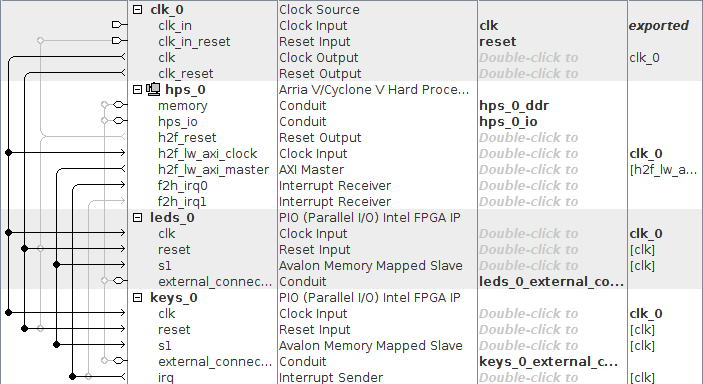
\includegraphics[scale=0.9]{img/quartus3.png}
\caption{Blok šema sistema}
\label{slika:q3}
\end{figure}

\subsection{Memorijski mapiran interfejs ka LE diodama i tasterima u FPGA}
Za projektovanje hardvera u FPGA koristi se PIO (\textit{Parallel Input/Output}) Intel FPGA IP blok. Ovo je jedan od mnogih dostupnih Intelovih IP blokova sa standardizovanim \textit{Avalon Memory Mapped Slave} interfejsom. HPS sistem pristupa registrima ovog IP bloka preko svoje standardne AXI magistrale. Između Avalon i AXI magistrale nalazi se automatski generisani \textit{brige}.

PIO Intel FPGA IP blok ima mogućnost da se konfiguriše kao ulazni, izlazni ili bidirekcioni. Takođe postoji mogućnost generisanja prekida na uzlaznu, silazni ili obe ivice ulaznog signala kao i mogućnost generisanja prekida na osnovu nivoa ulaznog signala. Dostupna su podešavanja za širinu paralelnog porta.

U tabeli ref su opisani registri PIO Intel FPGA IP bloka.

PIO Intel FPGA IP je u ovom radu iskorišćen za jednostavnu demonstraciju tako što je povezan na pinove Cyclone V sistema na čipu koji su na DE1-SoC razvojnom sistemu povezani na LE diode i tastere. U slučaju konkretne primene na rešavanje nekog problema, PIO Intel FPGA IP pruža jednostavan memorijski mapiran interfejs i mogućnost slanja prekida iz FPGA dela. Ova mogućnost korisna je u slučaju kada je za rešeavanje datog problema pogodno implementirati prizvoljno rešenje u pogramabilnoj logici. Ovaj pristup pruža slobodu projektovanja sistema u programabilnoj logici, a sa druge strane se zadržava standardizovani interfejs prema kompleksnom sistemu procesora. Na primer, izlazi PIO Intel FPGA IP registara mogu se koristiti kao konfiguracioni registri koji će upravljati korisničkom logikom, kao način da se pogramabilnoj logici dostave podaci koji će zatim biti obrađeni i vraćeni nazad. Mogućnost slanja prekida koristna je kada se PIO Intel FPGA IP koristi za posmartanje toka izvršavanja algoritma u programabilnoj logici - na promenu nekog signala se generiše prekid i opcioni zatim očitava iz statusnog regisra potrebna informacija koja oslikava stanje sistema. Takođe, prekid se može koristiti za sinhronizaciju toka podataka pri obradi podataka u FPGA tj. kao vid da se mikroprocesoru javi da su podaci spremni za čitanje. Rezultati rešavanja problema u FPGA se mogu učinti dostupnim spoljnom svetu preko nekog od mnogih standardnih interfejsa (USB, Ethernet, UART, ...) i to vrlo jednostavnim postupcima u okviru operativnog sitema na HPS delu.

U ovom projektu u FPGA delu su postavljena dva PIO (\textit{Parallel Input/Output}) Intel FPGA IP bloka. PIO IP blok \texttt{leds\_0} je izlazni i koristi se za kontrolisanje LE dioda. PIO IP blok \texttt{keys\_0} je ulazni i koristi se za očitavanje tastera. PIO IP blok \texttt{keys\_0} takođe šalje prekidni zahtev HPS-u na svaku uzlaznu i silaznu ivicu.

\subsection{Preloader}
Pri pokretanju HPS sistema koristi se \textit{preloader} generisan Alterinim alatima. Za generisanje \textit{preloader}-a neophodni su fajlovi za opis sistema koje generiše Platform Designer. Program za generisanje \textit{Preloader Generator} je deo Alterinog SOC EDS(\textit{Embedded Development Suite}) paketa alata. U grafičkom meniju se odabira folder u kojem se nalazi Platform Designer projekat sistema za koji se generiše \textit{preloader}. Ovako generisani \textit{preloader} je zasnovan na SPL (\textit{Secondary Program Loader}) \textit{framework}-u koji je deo U-Boot projekta. Ovo ima pozitivnu posledicu da \textit{preloader} i U-Boot dele dosta izvornog koda, kao što je mnoštvo pouzdanih drajvera.

Standardne funkcija \textit{preloader}-a za Cyclone V sistem na čipu su:
\begin{itemize}
\item inicijalizacija SDRAM interfejsa uključujići kalibraciju SDRAM PLL modula
\item dohvatanje \textit{bootloader} binarnog fajla sa \textit{flash} memorije (NAND, SD/MMC, NOR)
\item smeštanje binarnog fajla \textit{bootloader}-a u SDRAM i prepuštanje toka izvršavanja
\item konfiguriše multipleksiranje pinova(podešavanja za konfiguraciju su dostupna u Platform Designeru)
\item konfiguriše PLL na osnovu korisničkih podešavanja dostupnih u \textit{preloader generator}-u
\item otpušta određene periferije iz stanja reseta (izbor periferija se konfiguriše u Platform Designer-u)
\item inicijalizuje \textit{flash} kontroler (bilo NAND, SD/MMC ili QSPI) na osnovu \textit{boot} prekidača
\end{itemize}

U ovom radu se \textit{preloader} koristi za učitavanje U-boot \textit{bootloader}-a. U-boot \textit{bootloader} se nalazi na SD kartici. DE1-SoC razvojni sistem je već podešen za pokretanje sistema sa SD kartice, stoga je preostalo u \textit{preloader generator}-u uključiti podršku za \textit{FAT file system} i definisati ime binarnog fajla \textit{bootloader}-a. Nakon konfigurisanja \textit{preloader}-a potrebno je kompajlirati izvšni fajl koji će se prebaciti na razvojni sistem. Kompajliranje se vrši jednostavnim pozivom \textit{make} naredbe koja pokreće skriptu za \textit{make build system} koja kao rezultat daje izvršni fajl.

Ovaj izvršni fajl je potrebno prebaciti na SD karticu na posebnu particiju. Prilikom particionisanja SD kartice neophodno je predvideti ovu particiju i podesiti njen tip na posebnu vrednost \texttt{a2}.

\subsection{Bootloader}
\textit{Open-source} projekat U-Boot (\textit{Universal Boot Loader}) je uobičajeni izbor \textit{bootloader}-a za namenske sisteme zasnovane na ARM, PowerPC, MIPS procesorima. U-Boot se u ovom radu koristi za programiranje FPGA i učitavanje operativnog sistema. Ovo se postiže zahvaljujući tome što U-Boot nudi korisniku komandnu liniju koja se jednostavno može koristiti za pisanje skripti za željeno ponašanje \textit{bootloader}-a.

U-Boot se preuzima u obliku izvornog koda sa \texttt{git}-a[ref na git]
https://github.com/u-boot/u-boot
"Das U-Boot" Source Tree
Kako U-Boot podržava različite arhitekture potrebno je izvršiti konfiguraciju softvera. Konfiguracija je dostupna kao gotova za mnoge razvojne sisteme. Izvorni kod se konfiguriše kroz Kbuild infrastrukturu koja je se takođe koristi za konfiguraciju Linuksa. Konfiguraciju ovim putem se poziva iz komandne linije i pruža vrlo jednostavan grafički interfejs i veliku moć podešavanja.

Konfiguracija za DE1-SoC razvojni sistem je dostupna kao gotova, što znači da se lako dobija funkcionalno konfigurisan izvorni kod na jednostavan način. Osim toga, ovom konfigracijom dostupne su komande programiranja FPGA dela preko \textit{FPGA Manager} periferije.

Nakon osnovnog konfigurisanja softvera potrebno je napisati skriptu za željeno ponašanje i konfigurisanje U-Boot da pri pokretanju izvrši tu skriptu. Kroz Kbuild sistem se menja vrednost promenljive \textit{bootcmd} koja sadrži komandu koja će biti izvršena odmah po pokretanju sistema ukoliko korisnik ne prekine ovaj proces. Promenljiva \textit{bootcmd} je podešena tako da se izvrši kratka skripta za učitavanje naredne korisničke skripte (podešena je komanda \textit{run callscript}). Dalje, u izvornom kodu je na mestu predviđenom za korisničke definicije definisana jednostavna skripta \textit{callscript} koja samo učitava narednu korisničku skriptu (nazvanu \textit{u-boot.scr}). Na ovaj način je ostavljena sloboda za izmenu skripte i time ponašanja \textit{bootloader}-a bez potrebe da se ponovo konfiguriše i kompajlira U-Boot.

Ovim je konfiguracija U-Boot \textit{bootloader}-a završena i zatim se vrši kompajliranje kako bi se dobio izvršni fajl. Za kompajliranje koristi se besplatni \textit{Linaro toolchain}.
\subsubsection{Skripta za U-Boot}
Skripta za U-Boot piše se kao tekstualni fajl u skladu sa U-Boot sintaksom. U-Boot komande pružaju velike mogućnosti u cilju pokretanja operativnog sistema. Uobičajene mogućnosti ovih komandi su:
\begin{itemize}
\item podešavanje promenljivih okruženja operativnog sistema
\item dohvatanje binarnih fajlova za pokretanje operativnog sistema iz \textit{flash} memorije ili preko \textit{ethernet}-a pri čemu je omogućen pristup standardnim fajl sistemima kao i prenos preko mreže preko TFTP(\textit{Trivial File Transfer Protocol})
\item smeštanje binarnih fajlova za pokretanje sistema u SDRAM i prepuštanje toka izvršavanja
\item podešavanje \textit{boot} argumenata koja se koriste za podešavanje kernela operativnog sistema
\end{itemize}

Nakon pisanja skripte potrebno je \textit{mkimage} alatom dodati odgovarajući U-Boot heder. Fajl koji se dobija je potrebno prebaciti na SD karicu na FAT particiju. U-Boot je već konfigurisan pre kompajliranja tako da učita i izvrši ovu skriptu.

U ovom radu skripta je napisana tako da programira FPGA i pokrene Linuks operativni sistem. Fajlovi koje U-Boot čita pri izvršavanju ove skripte su:
\begin{itemize}
\item \texttt{socfpga.rbf} - binarni za konfiguraciju FPGA
\item \texttt{socfpga.dtb} - binarni fajl koji opisuje hardversku platofrmu za Linuks kernel
\item \texttt{zImage} - kompajlirani kernel
\end{itemize}

U skripti se podešava vrednost promenljive \texttt{bootargs} koja definiše argumente koji će biti prosleđeni kernelu pri pokretanju operativnog sistema. Ova promenljiva podešena je tako da definiše veličinu RAM memorije, parametre konzole za komunikaciju sa sistemom i određuje definisanu \texttt{ext3} particiju SD kartice kao \textit{root file system} Linuksa.

Nakon učitavanja ovih fajlova izvršavaju se sledeće važne komande:
\begin{itemize}
\item \texttt{fpgaload} - za programiranje FPGA
\item \texttt{bridge enable} - za inicijalizaciju AXI magistrale između FPGA dela i HPS dela
\item \texttt{bootz} - komanda za pokretanje pokretanje operativnog sistema pri čemu se kernelu prosleđuje \textit{Devie Tree Blob} i argumenti iz promenljive \texttt{bootargs}
\end{itemize}

\subsection{Device Tree}

\subsection{Linuks kernel i Root File System}
Izvorni kod za Linuks kernel je preuzet za Alterinog \texttt{git}-a. \textit{Root file system} je generisan korišćenjem \texttt{buildroot}-a i upisan na SD karticu.

\subsection{Drajver}
Drajver je napisan kao modul kernela koji se uključuje odgovarajućom komandom. Nakon uključivanja drajver iz binarnog opisa harvdera (\textit{Device Tree Blob}) učitava informacije o harvderu. Drajver pravi fajlove u \texttt{sysfs} fajl sistemu. Čitanje i upis u ove fajlove poziva odgovarajuće funkcije u drajveru koje upravljaju hardverom.

Sistemski fajlovi koje pravi drajver i njihov opis:
\begin{itemize}
\item \texttt{leds} - upisani broj se prikazuje na LE diodama u binarnoj predstavi
\item \texttt{keys} - čitanje vraća binarnu predstavu stanja tastera
\item \texttt{irq\_flag} - pristup registru za flegove prekida (1 na n-tom bitu označava pristigli prekid na n-tom tasteru, upis 1 na n-ti bit čisti n-ti fleg)
\item \texttt{irq\_mask} - čitanje i upis u registar za maksiranje prekida (upis 1 na n-ti bit omogućava prekid na n-tom tasteru)
\end{itemize}

Ceo kod drajvera je dostupan u dodatku.
\subsection*{Testiranje sistema}
Binarni fajlovi za pokretanje sistema i root fajl sistem su napisani na SD karticu. HPS je povezan sa PC računarom preko UART-USB serijske veze. Otvaranjem konzole na PC računaru se pristupa sistemu.\\
U nastavku je dat komplatan spisak koraka za realizovanje sistema.



